%\documentclass[11pt,a4paper,english]{report}
\documentclass[11pt,a4paper,english]{article}
\usepackage{babel}
\usepackage[utf8]{inputenc}
\usepackage{float}
\usepackage{color}
\usepackage{a4wide}
\usepackage{fancyhdr}
\usepackage{array,multirow,makecell}
\usepackage{amsmath,amsfonts,amssymb}
\usepackage{mathtools}
\usepackage{color}
\usepackage{multirow}
\usepackage{titletoc}
\usepackage{titlesec}
\usepackage[table,xcdraw]{xcolor}
\usepackage{MnSymbol,wasysym}
\usepackage{pdfpages}
\usepackage{afterpage}
\usepackage{hyperref}
\usepackage{verbatimbox}
\usepackage{graphicx}
\parskip 1ex
\parindent 0in

\renewcommand{\baselinestretch}{1.1}

%\setlength{\topmargin}{-0.7cm} \setlength{\textwidth}{16.4cm}
%\setlength{\textheight}{30cm} \setlength{\evensidemargin}{0cm}
%\setlength{\oddsidemargin}{-0.5cm} \setlength{\topmargin}{-1.5cm}

\setlength{\topmargin}{-0.8cm} \setlength{\textwidth}{16.4cm}
\setlength{\textheight}{25.5cm} \setlength{\evensidemargin}{0cm}
\setlength{\oddsidemargin}{-0.5cm} \setlength{\topmargin}{-1.5cm}

\begin{document}
		\renewcommand{\bibname}{Bibliography}
	
\begin{titlepage}
	\begin{figure}
		
\includegraphics[width=0.3\textwidth]{logo_IJCLab.jpg}
	\end{figure}
	 
	\centering
	\vspace{20cm}		
	\textit{ALERT software development.}
	
	\vspace{5cm}	
		
	\Large {\textbf { \textcolor{blue} {ALERT material budget and CLAS12 Drift Chamber occupancy.}}}
	
	\vspace{10cm}
	
	\Large{\textbf {Viktoriya Sergeyeva}}
	
	\today
	
	\vspace{1.5cm}
	\centering		
	\small { \textit {Laboratoire de Physique des 2 Infinis Irène Joliot Curie (IJCLab), CNRS, IN2P3 \\ 15 Rue Georges Clemenceau, 91400 Orsay}}	
\end{titlepage}

%\tableofcontents

\newpage

\section{ALERT material budget}
The goal of this study is to estimate the impact of non active materials on the resolution of CLAS12 with variables $\Delta P / P$, $\Delta \Theta$, $\Delta \phi$, $\Delta Z_v$. The mechanics of ALERT time of flight (ATOF) modules, the ribs, the upstream and downstream plates constitute the non active external shell. This shell encloses the target, ALERT drift chamber (AHDC) and ATOF. Several \textit{GEMC} simulations were performed considering different material configurations described below.
	\subsection{\textit{GEMC} simulations}
	Simulation without an external shell is taken as the reference. We only include the target, AHDC, ATOF and CLAS12 detectors such as: ctof, cnd, htcc, dc, ftof, ec, pcal, ltcc. We use "ft" with "FTOn" variation and "fc" with "TorusSymmetric" variation. Geant4 particle gun uses $e^{-}$ with $E = 4 \pm 3$ GeV, $\Theta = 15 \pm 10 ^{\circ}$, and $2\pi \ \phi$ range.
	
	Simulations including the external shell are compared to the reference. The shell consists of concentrical cylinders that enclose ATOF. Each layer corresponds to one material. There are back and front plates. The front (downstream) plate consists of discs of Macor, Cu and Al. All materials present in the external shell are: Al, PCB (nylon), C, steel, brass, Epoxy glass, Macor. Two updates were preformed since the initial version. The first one about ATOF parts changing from steel to Al, and the second one about changing 10 Al ribs by 10 Epoxy glass ribs. 
	To sum up, simulated configurations are:
	\begin{itemize}
		\item ATOF + AHDC only. External shell is not included - reference simulation.
		\item Initial external shell version (15 Al ribs, stainless steel presence)
		\item First material update: stainless steel eliminated, C added.
		\item Second materail update: 10 Epoxy glass\footnote{"EPOXY" composition is given by a mix \texttt{EpoxyOnly 0.35 SiO2 0.65}. Delmat Epoxy 68660.} and 5 Al ribs.
	\end{itemize}

	\subsection{Results}
Results were obtained by using the \texttt{kpp-plots} from \textit{Coatjava} package. It is possible to recover the simulated and reconstructed properties of the electrons (fig. \ref{fig_resol}).
The difference between the simulated and reconstructed values is computed and we obtain the  $\Delta P / P$, $\Delta \Theta$, $\Delta \phi$, $\Delta Z_v$ histograms. A gaussian is fitted for each histogram. Finally, we count how many events are outside the $\pm 2\sigma$ or $\pm 5\sigma$ intervals. The proportion of outside events is given in \% of total number of reconstructed events (tab. \ref{table_resol}).

\begin{table}[h!]
\centering
\begin{tabular}{|c|c|c|c|c|c|c|c|c|}
\hline
                  & \multicolumn{2}{c|}{\textbf{$\Delta P/P$}} & \multicolumn{2}{c|}{\textbf{$\Delta \Theta$}} & \multicolumn{2}{c|}{\textbf{$\Delta \phi$}} & \multicolumn{2}{c|}{\textbf{$\Delta Z_v$}} \\ \hline
                  & 2 $\sigma$         & 5 $\sigma$ & 2 $\sigma$          & 5 $\sigma$          & 2 $\sigma$         & 5 $\sigma$         & 2 $\sigma$         & 5 $\sigma$        \\ \hline
\textbf{no shell} & 25.7            & 15.2 & 17.2             & 5.5              & 16.7            & 8.2             & 11.8            & 3.2            \\ \hline
\textbf{initial}  & 41.3            & 29.2 & 23.5             & 7.4              & 28.8            & 14.6            & 12.7            & 3.6            \\ \hline
\textbf{update 1} & 41.5            & 29.7 & 23.35            & 7.4              & 29.0            & 14.9            & 12.8            & 3.5            \\ \hline
\textbf{update 2} & 41.7            & 29.7 & 22.7             & 7.1              & 28.3            & 14.7            & 12.9            & 3.5            \\ \hline
\end{tabular}
\caption{Proportion of $\pm 2 \ and\ \pm5 \sigma$ outside events (\% of total number of reconstructed events).}
\label{table_resol}
\end{table}

The addition of the external shell increases the number of outside events by a factor of 1.7 - 1.1 depending on the variable. Smallest variation is for $\Delta Z_v$. Material choices for the construction are being ajusted in order to minimize the external shell impact. 

\begin{figure}[h!]
\centering
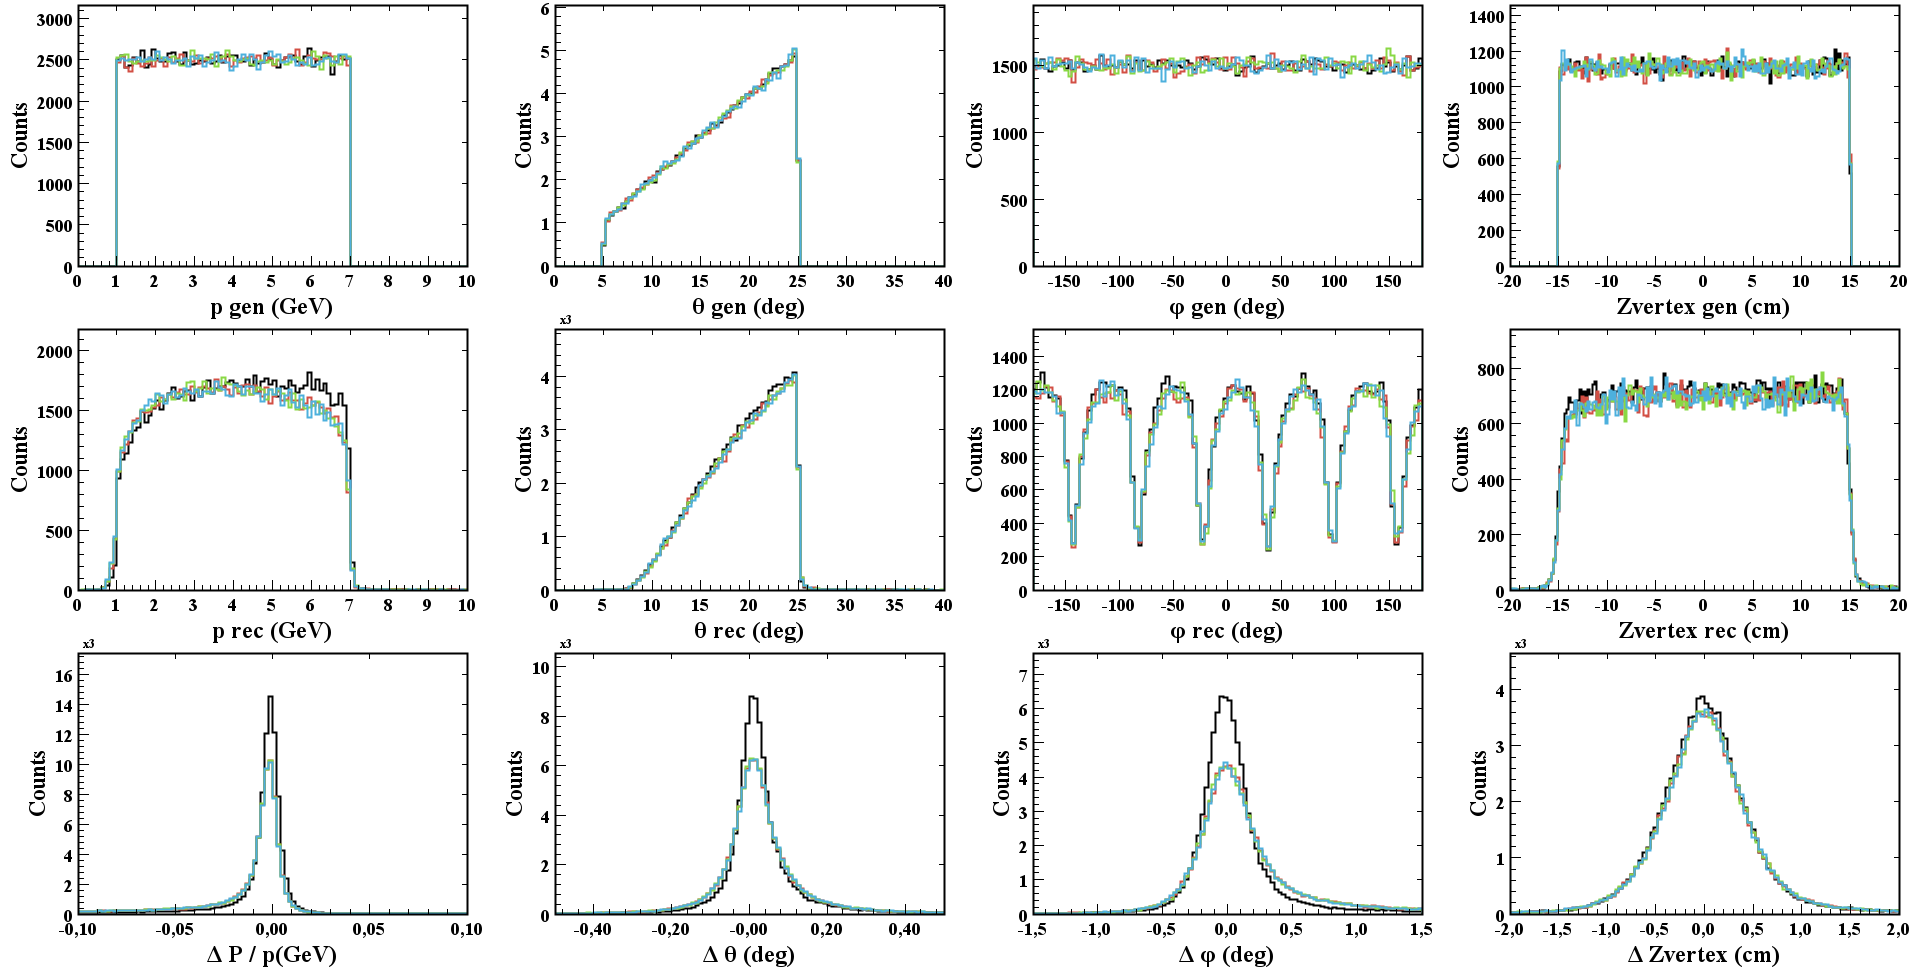
\includegraphics[width=1.0\textwidth]{generated_reconstructed_variables_MC.png}
%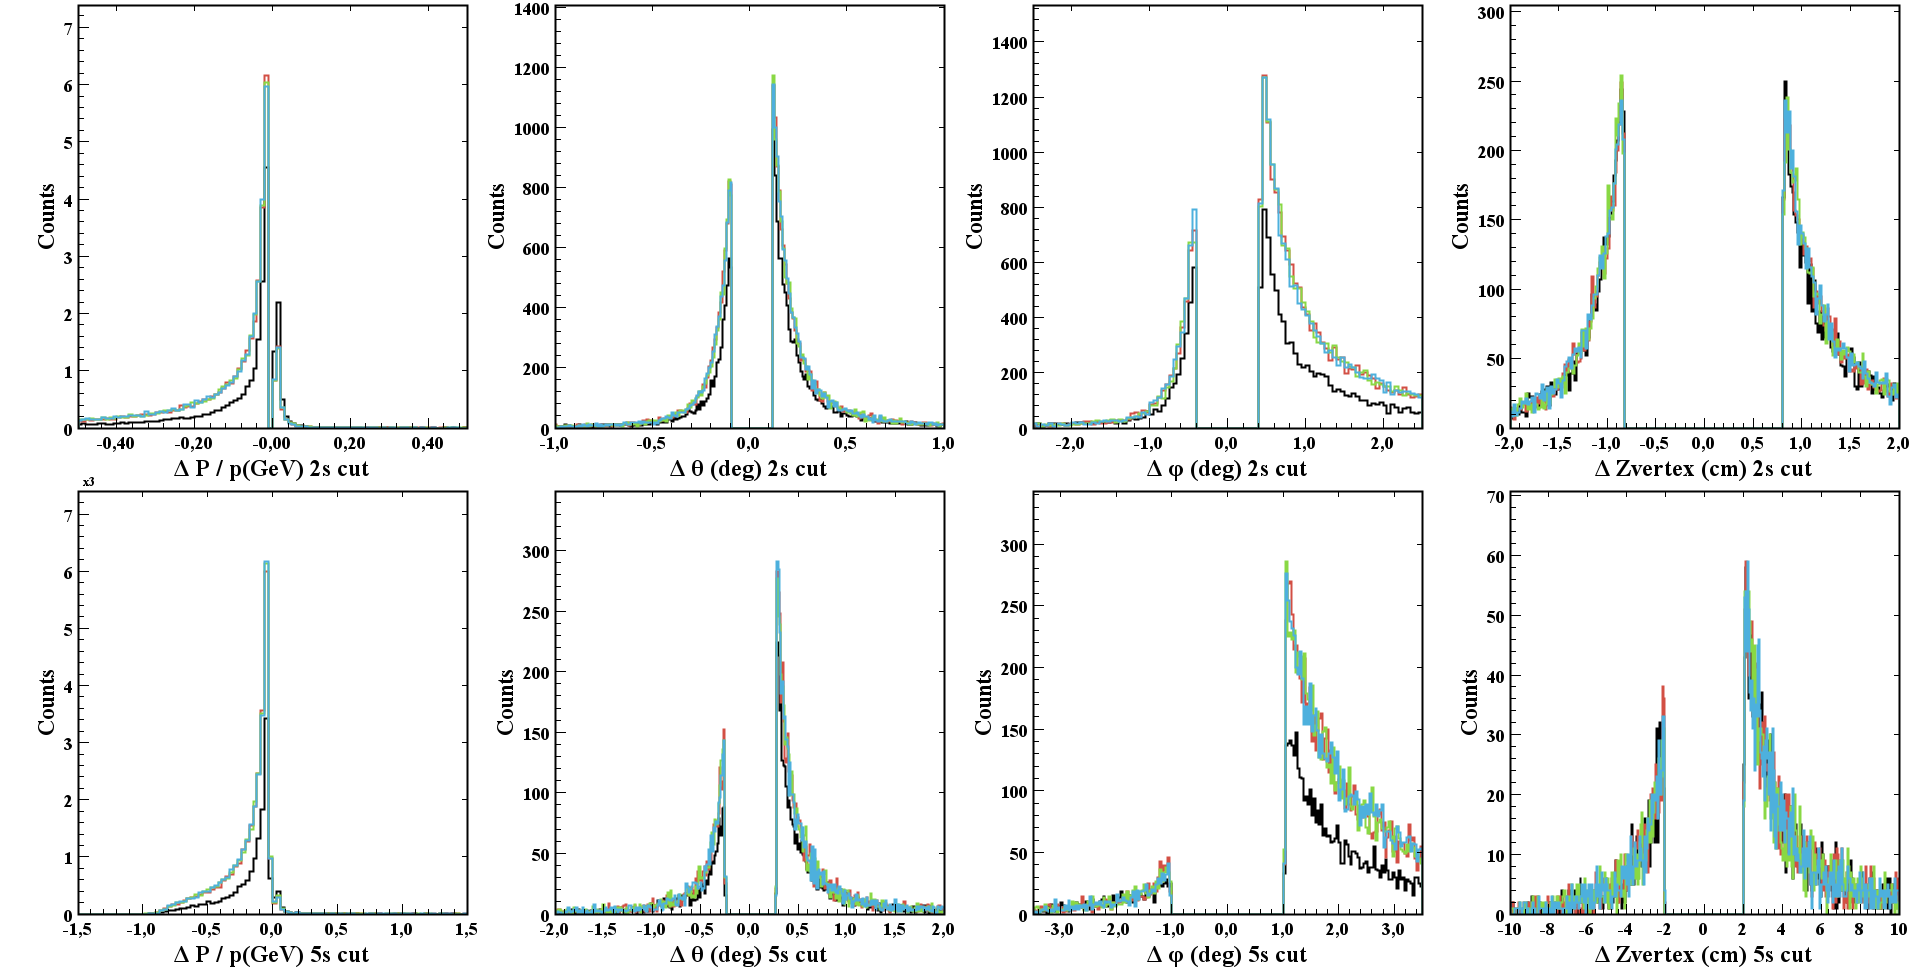
\includegraphics[width=1.0\textwidth]{variables_MC_cuts_2and5sigma.png}
\caption{$P,\ \Theta,\ \phi,\ Z_v$ for simulated and reconstructed events.}
\label{fig_resol}
\end{figure}

Finally, in order to have more details about geometry impact on the resolution, we devided $Z$ and $\Theta$ in 2 parts:
\begin{itemize}
	\item $Z$ axis - $[-20, 0)$ and $[0, 20]$ cm, that we call here $Z^{-}$ and $Z^{+}$.
	\item $\Theta$ angle - $[5, 15)$ and $[15, 45]$ degrees, that we call here $\Theta_{low}$ and $\Theta_{high}$
\end{itemize}
We can obtain 4 combinations with these spatial divisions. We count, as before, the number of reconstructed events outside the $\pm 2 \sigma$ interval and we compute the $\%$ with the respect to the total number of reconstructed events inside a given interval of $Z, \ \Theta$. We compare the reference setup "no shell" (table \ref{table_grid_noshell}) to the last configuration "update 2" (table \ref{table_grid_update2}).
We notice that $Z^{-} \Theta_{high}$ region is the one that contributes the most to the number of outside events. 
The resolution of $\Delta Z_v$ does not change drastically when we go from one region to another.

\begin{table}[h!]
\centering
\begin{tabular}{|c|c|c|c|c|}
\hline
                     & \textbf{$Z^{-} \Theta_{low}$} & \textbf{$Z^{-} \Theta_{high}$} & \textbf{$Z^{+} \Theta_{low}$} & \textbf{$Z^{+} \Theta_{high}$} \\ \hline
\textbf{$\Delta P/P$}   & 20.6                  & 32.9                   & 18.6                  & 20.6                   \\ \hline
\textbf{$\Delta \Theta$} & 10.05                 & 17.4                   & 13.1                  & 16.6                   \\ \hline
\textbf{$\Delta \phi$}   & 12.5                  & 21.3                   & 14.6                  & 13.6                   \\ \hline
\textbf{$\Delta Z_v$}    & 12.8                  & 12.7                   & 12.8                  & 12.3                   \\ \hline
\end{tabular}
\caption{Proportion of $\pm 2\sigma$ outside events (\% of total number of reconstructed events) for "no shell" configuration.}
\label{table_grid_noshell}
\end{table}

\begin{table}[h!]
\centering
\begin{tabular}{|c|c|c|c|c|}
\hline
                     & \textbf{$Z^{-} \Theta_{low}$} & \textbf{$Z^{-} \Theta_{high}$} & \textbf{$Z^{+} \Theta_{low}$} & \textbf{$Z^{+} \Theta_{high}$} \\ \hline
\textbf{$\Delta P/P$}   & 39.4                  & 53.1                   & 25.7                  & 33.0                   \\ \hline
\textbf{$\Delta \Theta$} & 20.2                  & 24.3                   & 17.9                  & 22.6                   \\ \hline
\textbf{$\Delta \phi$}   & 26.8                  & 37.4                   & 19.1                  & 24.0                   \\ \hline
\textbf{$\Delta Z_v$}    & 14.8                  & 14.4                   & 13.8                  & 12.9                   \\ \hline
\end{tabular}
\caption{Proportion of $\pm 2\sigma$ outside events (\% of total number of reconstructed events) for "update 2" configuration.}
\label{table_grid_update2}
\end{table}




\newpage
\section{CLAS12 Drift Chamber occupancy}
The goal of this study is to compare CLAS12 Drift Chamber (DC) occupancy for ALERT luminosity and target with occupancy levels for standard CLAS12 luminosity and liquid $H_2$ target. Maximum value for ALERT beam current is 650 nA whereas usual occupancy studies in CLAS12 are for $I_{max} \approx 80$ nA. Results were obtained by \texttt{dcc\_occ} .root macro using Monte Carlo truth from CLAS12 DC banks. This is the standard method for such study in the collaboration.

	\subsection{\textit{GEMC} simulations}
The simulation includes:
\begin{itemize}
	\item AHDC + ATOF and their external shell.
	\item $300$ mm long target filled with $D$ gas at $5$ atm., $G4\_Al$ 0.03 mm downstream and upstream windows, 0.060 mm $G4\_KAPTON$ target wall.
	\item He bag in $G4\_Al$ and $G4\_He$, between the target and the beamline.
	\item CLAS12 detectors, magnets and beamline elements.
\end{itemize}
Time window used for all simulations is 250 ns. ALERT highest current $650$ nA is equivalent to: $N_{electrons} = I*6.24\times 10^{18} \ (charges/s) *T_ {window} \ (s) = 1014357$. Long simulations were performed to have at least 10000 events for estimation study. We have also performed simulations without the external shell and without He bag to see the impact on DC occupancy.

In case of standard liquid $H_2$ target, we use $N_{electrons} = 124000$. 

	\subsection{Results}
CLAS12 DC occupancy is given for each of 3 regions. Figure \ref{fig_occ_alert} shows the occupancy for ALERT configuration and luminosity. For the standard liquid $H_2$ target, figure \ref{fig_occ_standardLH2} shows slightly higher occupancy levels than for ALERT configuration. Finally, figure \ref{fig_occ_noShellNobag} shows the advantage, in terms of occupancy, of adding He bag since the setup without the external shell and He bag gives even higher DC occupancy.   

Since we observe that DC occupancy for ALERT luminosity and configuration is under the occupancy for the standard liquid $H_2$ target, we estimate that our configuration is satisfactory.
\begin{figure}
\centering
\includegraphics[width=0.6\textwidth]{/vol0/viktoriya/Bureau/IPNO_teletravail/LaTex_docs/ALERT_DCoccupancy_checks/January_2021/ALERT_config_occ_plots/dc_region_occ.pdf}
\caption{CLAS12 DC occupancy for ALERT luminosity and setup. $N_{electrons} = 1014357$.}
\label{fig_occ_alert}
\end{figure}

\begin{figure}
\centering
\includegraphics[width=0.6\textwidth]{/vol0/viktoriya/Bureau/IPNO_teletravail/LaTex_docs/ALERT_DCoccupancy_checks/January_2021/standard_LH2target/dc_region_occ.pdf}
\caption{CLAS12 DC occupancy for standard liquid $H_2$ target. $N_{electrons} = 124000$.}
\label{fig_occ_standardLH2}
\end{figure}

\begin{figure}
\centering
\includegraphics[width=0.6\textwidth]{/vol0/viktoriya/Bureau/IPNO_teletravail/LaTex_docs/ALERT_DCoccupancy_checks/January_2021/no_shell_no_Hebag_bckgStudy/dc_region_occ.pdf}
\caption{CLAS12 DC occupancy for ALERT luminosity, $\nexists$ shell, $\nexists$ He bag. $N_{electrons} = 1014357$.}
\label{fig_occ_noShellNobag}
\end{figure}



%\newpage	
%\section{Conclusions}
%... \\

%bla bla bla \\

%...

\end{document}